\chapter{Methods}\label{chapter:Methods}

To answer the research questions from section \ref{section:Research_Questions}, we formed three approaches.
To answer the question ``What is the current state of language workbenches supporting projectional editing?'', we carried out a Systematic Literature Review, which we describe in section \ref{section:Method_systematic_review}.
We followed two linked approaches for the question ``Which projections can help developers get appropriate feedback about rules?''.
Firstly, using Action Design Research (ADR), we implemented Drools as a projectional editor, and then some projections that users can edit.
Then, we presented our findings to experienced Drools users through a questionnaire survey to validate this approach.

\section{Method: Systematic Review}\label{section:Method_systematic_review}

To answer the first Research Question, ``what is the current state of Projectional Editing?'', we conducted a systematic literature review.
Hereafter, we describe the method we undertook.

To carry out this review we followed Kitchenham's\cite{Kitchenham_2015} advice on systematic review protocol validation, (see appendix \ref{appendix:protocolValidation} for the exact checklist we used).

\subsection{Motivation}
The motivation that preceded this research was a requirement to understand if projectional editing was an idea that was worth investigating.
Through our background research we saw an interest in the precursors to projectional editing in the late 70's through to the mid 80's.
This seemed to be abandoned until the mid 90's following Charles Simonyi's treaties on Intentional programming.
This did not lead to a swell in academic research as his companies product, Intentional Domain Workbench was a closed commercial product.
There seemed to be a burst of academic interest after the release of JetBrain's OpenSource Meta Programming System (MPS) in the late 2000's.

Is there a need for a study of this topic? 
We believe, at least in the microcosm of this master's project it is helpful to know whether we are researching in an area that is dying of vibrant.

For the wider community, there does not seem to be any systematic reviews specifically about projectional editing, let alone recently.
This study is not extending any previous Systematic Review as, although there were literature surveys and mapping studies covering some adjacent fields, no SLRs were found.
Thus we believe it may be useful for those in the language engineering research community to bring together all current research in the area of projectional editing in one place.

\subsection{Research Question}
This paper we only have one research question to synthesize the findings of scientific papers towards.
This is ``What is the current state of Projectional Editing?''

This question for us can be broke down into:
\begin{itemize}
    \item \textbf{Sub Question 1} ``Is there current research in the area of projectional editing?''
    \item \textbf{Sub Question 2} ``What tools are currently being used for research?''
    \item \textbf{Sub Question 3} ``What is the sentiment in papers currently discussing projectional editing?''
\end{itemize}


\subsection{Search Strategy}

The search process is automated as SLRs require a high level of completeness, which cannot be effectively achieved manually.
Our first major decision was whether to engage in creating a quasi-gold standard as advised by Zhang\cite{Zhang_2011}.
Zhang noted that the ad-hoc nature of search strategies in SLRs has limitations.
We executed a preliminary ad-hoc search to try and ascertain the extent of the research space.
Upon satisfying ourselves that it was small enough, we rejected the Quasi-Gold standard as overkill for our requirements.

The search terms we landed on were as follows:
{\obeylines\obeyspaces
\texttt{
    ``PROJECTIONAL EDITING'' 
       OR 
    ``PROJECTIONAL EDITOR'' 
}}

This is to be adjusted to fit the query syntax of the various search engines.

As most Research Search engines offer the option of date ranges, and to save the effort of excluding later we also used the date range to eliminate unnecessary paper at the automated search stage.
Our research question we are specifically looking at the current state of projectional editing.
A design decision of many research search engines is that date ranges can often only be defined in whole years.
When designing our search strategy, it was near the beginning of 2021, and thus we feared that this would be too small a search space, thus we set our date range to be from the beginning of 2020 to present.
For the sake of reproducibility, it is advised to remove any papers after 31st July 2021.

The Search Engines used are shown in table \ref{table:searchEngines}.

\begin{table}[H]
    \begin{center}         
        \begin{tabular}{|l||l|}
            \hline
            ACM digital library       & Google Scholar       \\
            \hline
            BASE                      & CORE                 \\
            \hline  
            IEEE Xplore               & ISI Web of Science   \\
            \hline  
            Microsoft Academic        & Science.gov          \\
            \hline  
            Wiley InterScience        & SCOPUS               \\
            \hline  
            Semantic Scholar          & SpringerLink         \\
            \hline  
        \end{tabular}
    \end{center}
    \caption{Search Engines Used}
    \label{table:searchEngines}
\end{table}

Once we have filtered the automated search through the criteria of the selection stage, we will use that as our starting set for snowballing.
Our filtering will be done before the quality of the papers has been assessed, as we feel that excluding papers on quality of primary study issues may artificially limit the network of potential papers.
Our snowballing procedure shall follow the advice of Wohin\cite{Wohlin_2014}.
This is the idea of using the reference lists from our start set and applying the same selection criteria to these.

Where possible we will get the forward snowballing papers from the ``cited by'' functionality of Google Scholar.
Because of the range of the search being to present, all papers that cite the target paper will fall within our criteria.
For backward snowballing we will manually filter the bibliography section of the selected papers, selecting any paper published in 2020 or 2021

After gathering all the papers from the forward and backward snowballing we will again apply the selection criteria.
This process will iterate recursively until no new papers are found.
All of the papers not excluded in each iteration will be the basis for the quality of primary studies filtering stage.

After the final iteration, as a final step the selected papers will have a deeper scan.
This is to verify our initial scan that the papers met our inclusion criteria, before moving on to the quality assessment.

\subsection{Study Selection}

The inclusion criteria are:
\begin{itemize}
       \item Studies are about or mention projectional editing or one of it's synonyms
       \item It is published in during the period 2020\-2021
\end{itemize}

The exclusion criteria are:
\begin{itemize}
       \item Books and grey literature
       \item not English
       \item no full text available
       \item papers with serious issues with grammar or vocabulary
       \item not a previously selected paper
       \item not a paper about a previously reported on study
\end{itemize}

If multiple papers look at the same study with different approaches, then the data will be aggregated in the synthesis stage.

As a lone researcher, we must be aware of bias in positively including relevant papers and excluding irrelevant papers.
We will follow Kitchenham's suggestions to overcome such bias:
\begin{itemize}
       \item Test-retest 
       \begin{itemize}
              \item We will assess the papers once (on title abstract and keywords) against the inclusion and exclusion criteria.
              \item Save all the suggested results
              \item Assess the papers again three days later in a different order to the first  
       \end{itemize}
       \item If there are disagreements, we will use Cohen's Kappa agreement statistic\cite{Cohen_1960} to see if the process needs to be refined.
\end{itemize} 

If our searches appear to be too large for a lone researcher, we will turn to text mining.
We will be cautious to use this.
O'Mara-Eves et al.'s systematic review of text mining in systematic reviews\cite{OMara-Eves_2015}, recommends that this can be used for prioritization, but finds that for exclusion screening, although promising, it is not yet proven.

An SLR is interested in studies rather than papers.
There is a many-to-many relation between papers and studies.
We will review the selected papers to note when this has happened in our results to make sure studies do not get over or undercounted.

\subsection{Quality of Primary Studies}
To discover explanatory reasons for why there may be differences in study results, and to weigh how valuable specific studies are, we will assess the quality of the selected studies.

To try and avoid a Results Section bias we will be operating a results-blind quality assessment.
Study quality will be based on the methods section of the papers only.
This bias is threatened because results are summarized in the abstract.
The study quality will not be measured until after the selection process is complete, though it will, in part be carried out before the selection re-test.
list of papers will be randomly sorted before assessing for quality.

For EBM studies there are some well-known hierarchies of evidence for study quality thresholds such as the CRD Hierarchy of Evidence\cite{Cochrane_2019}.
Kitchenham in, Procedures for Performing Systematic Reviews\cite{Kitchenham_2004_2}, suggests the hierarchy shown in table \ref{table:hierarchy}

\begin{table}[H]
    \begin{center}   
    \resizebox{\textwidth}{!}{%
      
        \begin{tabular}{|l||l|}
            \hline
            Rank     & Description                                                                                         \\
            \hline
            \hline
            1        & Evidence obtained from at least one properly designed randomized controlled trial                   \\ 
            \hline  
            2        & Evidence obtained from well-designed pseudo-randomized controlled trials                            \\
                     & (i.e. non-random allocation to treatment)                                                           \\
            \hline  
            3-1      & Evidence obtained from comparative studies with concurrent controls and allocation not randomized,  \\
                     & cohort studies, case-control studies or interrupted time series with a control group                \\
            \hline  
            3-2      & Evidence obtained from comparative studies with historical control, two or more single-arm studies, \\
                     & or interrupted time series without a parallel control group                                         \\
            \hline  
            4-1      & Evidence obtained from a randomized experiment performed in an artificial setting                   \\
            \hline  
            4-2      & Evidence obtained from case series, either post-test or pre-test/post-test                          \\
            \hline  
            4-3      & Evidence obtained from a quasi-random experiment performed in an artificial setting                 \\
            \hline  
            5        & Evidence obtained from expert opinion based on theory or consensus                                  \\
            \hline  
        \end{tabular}}
    \end{center}
    \caption{Study design hierarchy for Software Engineering}
    \label{table:hierarchy}
\end{table}

These different types of study have different quality assessment criteria.
As the nature of our research questions is not likely to attract randomized or pseudo-randomized controlled trials or experiments, our quality assessment checklists are created with comparative studies and case series in mind.
To assess the strength of each primary study we used the checklists shown in appendix \ref{appendix:QualityAssesmentChecklist}.
The checklists were based on a subset of the questions suggested in Keele's guidelines on SLRs\cite{keele2007guidelines}, which in turn extracted questions from previous mostly medical systematic reviews.
Where necessary the selected questions were modified for software engineering.

These checklists are addressed toward general research.
In Software Engineering many studies that fall under what Gregor\cite{gregor2006nature}, in ``A Taxonomy of Theory Types in Information Systems Research'' calls ``Type V: Theory for Design and Action''.
The checklists do not address this type of research well.
On investigation into how others SLRs conduct quality assessment we did not find a solution to this issue.
Therefore we will continue with the checklists as in the appendix, using the checklists for Case Study for Type V research papers.
We will take this into account before dismissing results of this type on basis of their quality score.

As this study will be carried out by a lone researcher, there is no need to have a process for disagreements.
To check on the bias, several papers will be randomly selected and assessed using the checklist by the academic and the daily supervisors.
Should there be a high disagreement the design of the checklist will be revisited.

The quality checklist is trying to weed out the biases of selection, performance, detection, and exclusion, as well as other threats to the validity of the studies under test.
Validity issues can occur during the design, operation, analysis, or conclusion of an empirical study.

\subsection{Data Extraction}
No data extraction will be necessary for the first sub-question,  ``Is there current research in the area of projectional editing?''.
The fact of the existence of papers that have been verified to be primary studies either into projectional editing theory or practical use of it will be enough to answer the question.

For the question of ``What tools are currently being used for research?'', we shall note each tool discussed specifically with regards to the study being carried out.

Finally, for the sentiment we shall pass each paragraph of the introduction, the discussion and the conclusion through a sentiment analyser and, if the paragraph is pertinent to projectional editing, we will not it's sentiment score.
The sentiment analysis tool we shall use is Microsoft Azure Cognitive Services Text Analytics.
The code to carry out this task is shown in listing \ref{listing:text_analytics}

\begin{lstlisting}[language=Python, caption=Text Analytics code., captionpos=b, label=listing:text_analytics, breaklines=true]

    from azure.core.credentials import AzureKeyCredential
    from azure.ai.textanalytics import TextAnalyticsClient
    
    endpoint = "REPLACE_WITH_CORRECT_ENDPOINT"
    key = "REPLACE_WITH_CORRECT_KEY"
    
    text_analytics_client = TextAnalyticsClient(endpoint=endpoint, credential=AzureKeyCredential(key))
    
    inputfiles = [[ARRAY_OF_FILES_TO_BE_ANALYSED]]
    
    with open('/content/sample_data/sentiment/output_all.txt','a') as outf:
      for sections in inputfiles:
        for section in sections:
          print("Section: {}".format(section),file=outf)
          f = open('/content/sample_data/sentiment/'+section)
          content = f.readlines()
          # for brevity an optimization to deal with 10 document limit is removed
          if len(content) != 0:
            result = text_analytics_client.analyze_sentiment(content, show_opinion_mining=True)
            docs = [doc for doc in result if not doc.is_error]
            for idx, doc in enumerate(docs):
              print("sentiment: {}".format(doc.sentiment),file=outf)
              print("Document text: {}".format(content[idx]),file=outf)
\end{lstlisting}


\begin{table}[H]
	\centering
	\begin{tabular}{|c | l | l | c |} 
		\hline
		\#& Data Type           & Description                                          & RQ     \\ \hline
		\hline
        1 & Study ID            & Unique identifier for the study                      &        \\ \hline
        2 & Title of Study      & The paper name                                       &        \\ \hline
        3 & Year of Publication & Will be either 2020 or 2021                          &        \\ \hline
        4 & Author(s) Names     & Including affiliation                                &        \\ \hline
        5 & Source of Study     & Name Of Online Database/ Digital Library             &        \\ \hline
        6 & Type of Study       & Publication/Conference/Workshop/Symposium            &        \\ \hline
        7 & Name of Venue       & Journal/Conference in which study has been published &        \\ \hline
        8 & Tools in Study      & A list of the tools used                             & RQ 1.2 \\ \hline
        9 & Sentiment           & The sentiment scores from appropriate paragraphs     & RQ 1.3 \\ \hline		
	\end{tabular}	
	\caption{Data extraction form.}
    \label{table:Data_Extraction_Form}
\end{table}

\subsection{Data aggregation and synthesis}
As explained by Kitchenham\cite{kitchenham2015evidence}, in software engineering, primary studies will tend to be too heterogeneous for any statistical analysis.
Synthesizing outcomes from multiple methods will be difficult.
Thus our synthesis will take a narrative approach.

Narrative synthesis is telling a story of the who, how, and why of the success or otherwise of the research.
For ADR research, focus will be on what will help or hinder the adoption of the implementations.
It will also examine how reliable the results are and relationships between the studies.


\newpage
\section{Method: Action Research - Drools in MPS}\label{section:Method_action_research}

Even though Drools is a relatively small DSL, we did not feel the need to implement all of the functionality to answer our questions.

\subsection{Really Simple Rules Language}
As we were new to DSL design and MPS, we First would create a very simple approximation of the Drools language with which to create our first projections.
We called this language "Really Simple Rules" (RSR).

\paragraph{File} RSR, Like Drools itself, has a File as it's root node.
The file only contains Facts and Rules.

\paragraph{Fact and FactProperty} In Drools a fact represents a Java Bean with its subsequent properties which can also be types with their own properties.
In RSR we limited properties to only allow boolean values.
This decision was based on the fact selection is a predicate and thus can only return a boolean.
By only having booleans we also limit the operations on the property.

\paragraph{Rule} For the Rules Concept, we decided to only simulate the Left Hand Side, or "When" conditions", of a Drools Rule.
We believed this would be enough to provide us with interesting projections, and did not want to over complicate this first approach.
An RSR Rule consists of a collection of conditions. 
Should all those conditions return true then the rule is selected.

\paragraph{Condition} A condition operates on one or more FactSelectors.
There are four condition type Exists, Not, And, and Or.
Exists and Not are unary conditions and evaluate one FactSelector.
And and Or evaluate two Fact Selectors.

\paragraph{FactSelector} a FactSelector consists of a reference to a Fact and a collection of Predicates.
If the Fact exists and all the predicates evaluate to true then the fact selector evaluates to true.

\paragraph{Predicate} the predicate is an operation on a fact property, to which the concept has a reference.
As the fact property represents a boolean value, then the only predicate operations are ``Is'' and ``Not''.

Figure \ref{fig:RSRDiagram} shows the Concept hierarch for this very simple implementation.

\begin{figure}[h]
    \centering
    \fbox{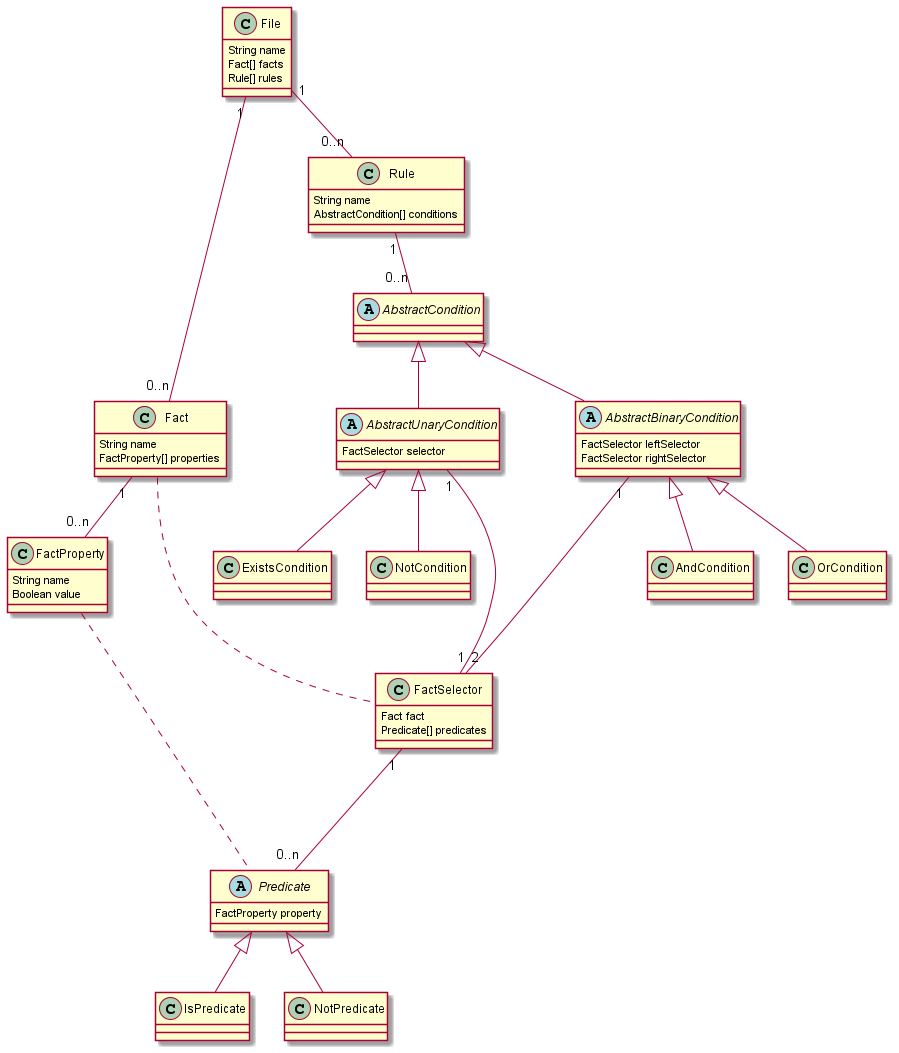
\includegraphics[width=0.95\textwidth]{Sections/images/ReallySimpleRuleLanguage.png}}
    \caption{RSR Concept Hierarchy}
    \label{fig:RSRDiagram}
\end{figure}

This design was then realised in MPS.
As the aim is to attempt different projections we did not initially optimise for editing.
The structure is as show in figure \ref{fig:RSRStructure} and the editors including those shown in figure \ref{fig:RSREditors}.

\begin{figure}
    \centering
    \begin{minipage}{0.30\textwidth}
        \centering
        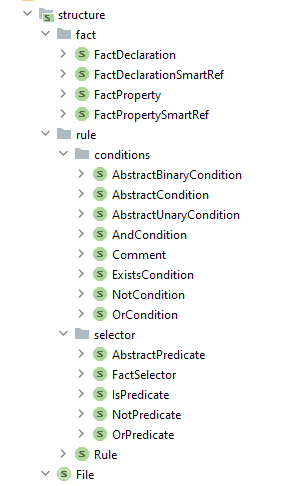
\includegraphics[width=0.9\textwidth]{Sections/images/RSRStructrure.png}
        \caption{RSR}
        \label{fig:RSRStructure}
    \end{minipage}\hfill
    \begin{minipage}{0.70\textwidth}
        \centering
        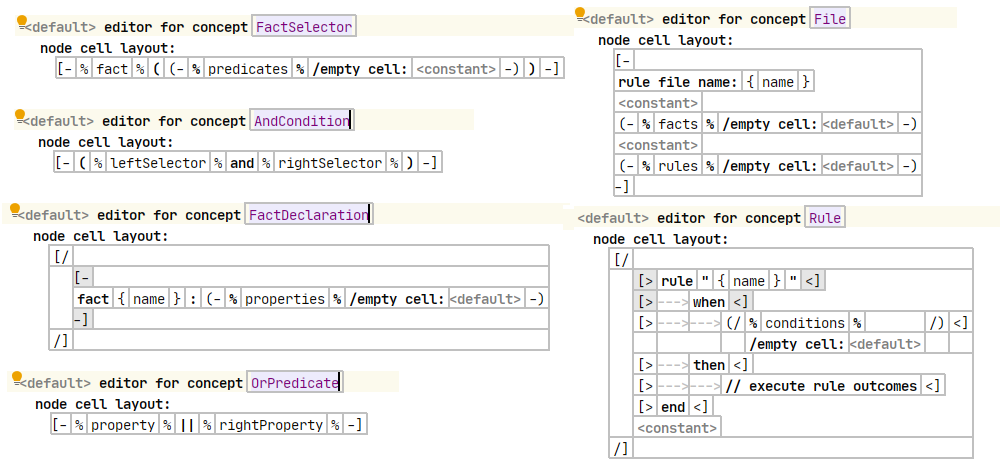
\includegraphics[width=0.9\textwidth]{Sections/images/RSREditors.png} 
        \caption{Editors}
        \label{fig:RSREditors}
    \end{minipage}
\end{figure}

Part of the research question is using projections to reason about large files.
In order to answer this we needed to simulate a large file.
To do this we had to enter a large number of rules.
As this becomes tedious we added a number of editing aids including substitute menus to speed up the entry of conditions, as shown in figure \ref{fig:RSRSubstituteMenu}.
This image, shows that before I had to select an ExistsCondition concept, and thereafter select the Fact for the condition.
After adding the substitute menu, I could immediate select the Fact I wanted and it would then automatically be wrapped with an ExistsCondition node. I could immediatly select the Fact and the 

\begin{figure}[h]
    \centering
    \fbox{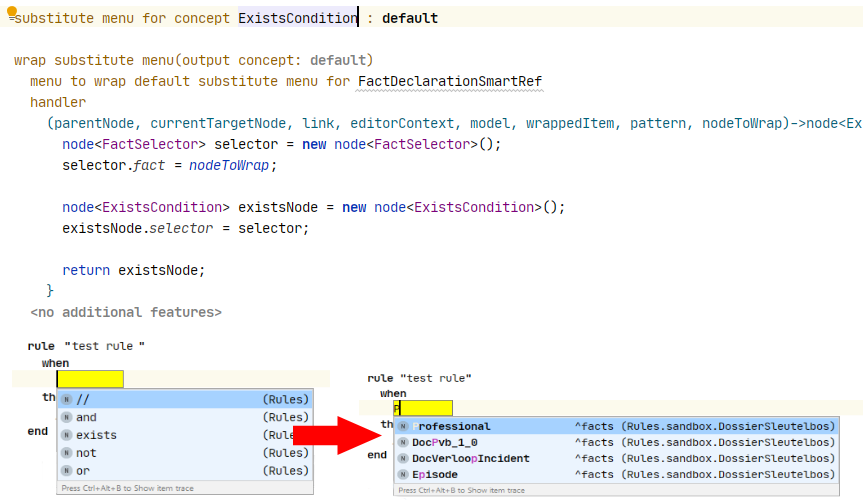
\includegraphics[width=0.95\textwidth]{Sections/images/RSRSubstituteMenu.png}}
    \caption{RSR Substitute Menu}
    \label{fig:RSRSubstituteMenu}
\end{figure}

We also added some intentions to invert incorrectly added conditions.

Finally, we added a constraint to scope the fact properties in predicates to the Fact chosen in the FactSelector.
This made it much easier to select properties in the predicates as indicated in figure \ref{fig:RSRConstraint}.
In the figure you can see that before the scoping constraint it showed a list with dozens of potential FactProperties, that represented all the FactProperties in the Model.
After the constraint is added it only shows the two properties associates with the Fact from the FactSelector.

\begin{figure}[h]
    \centering
    \fbox{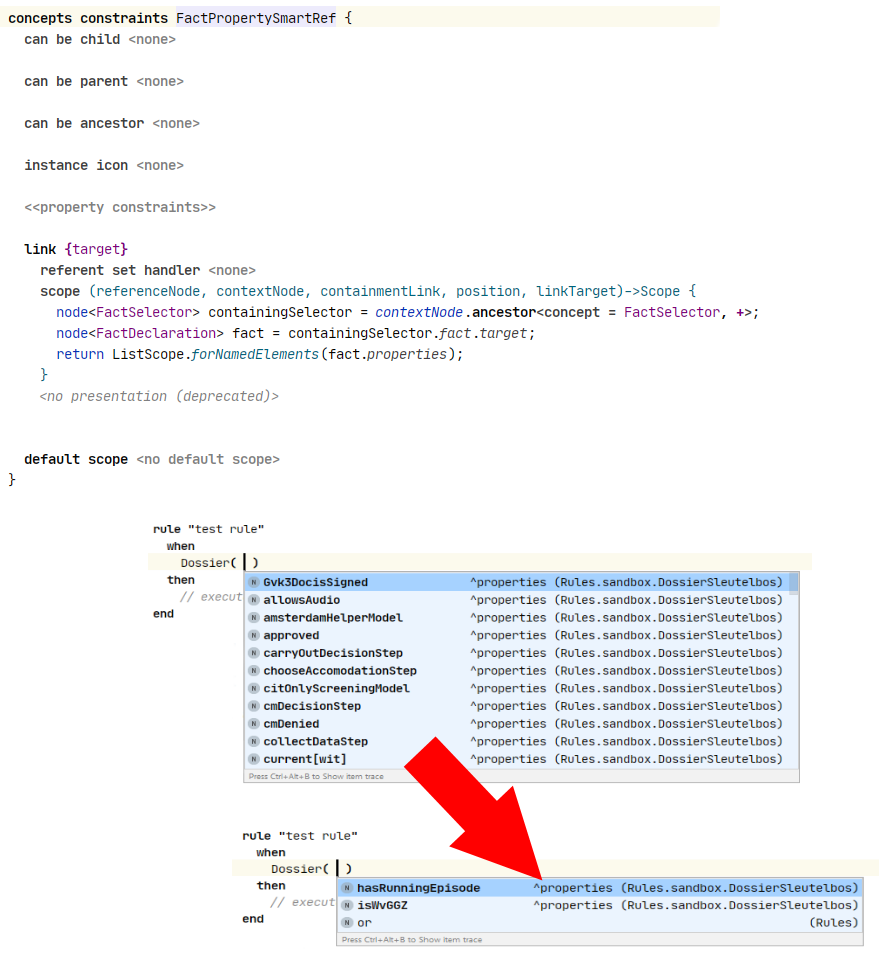
\includegraphics[width=0.95\textwidth]{Sections/images/RSRConstraint.png}}
    \caption{RSR Scoping Constraint}
    \label{fig:RSRConstraint}
\end{figure}

Thus, we have described the entire implementation of the Really Simple Rules Language.

After implementing the language we wrote a program with a large number of rules.
This program on which we will experiment with the different projections.
An example of our default Drools like text projection is show in figure \ref{fig:RSRProgram}.

\begin{figure}[h]
    \centering
    \fbox{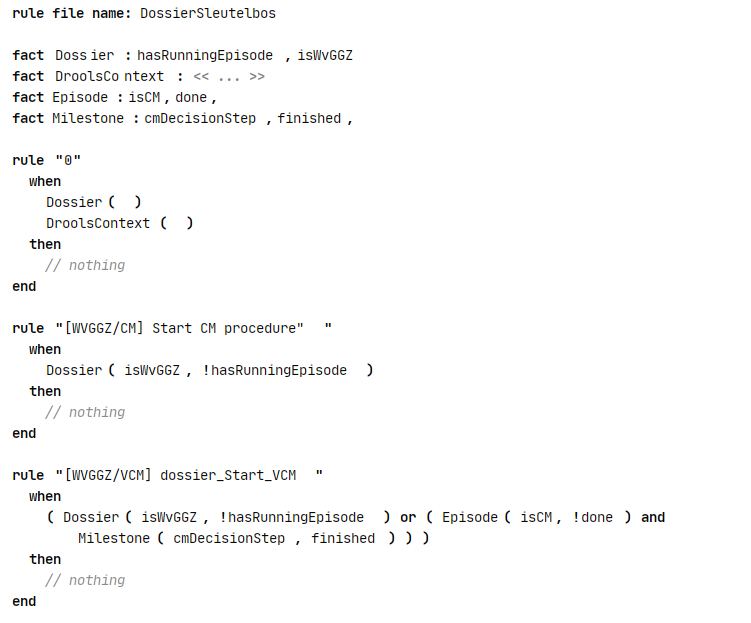
\includegraphics[width=0.95\textwidth]{Sections/images/RSRProgram.png}}
    \caption{RSR program}
    \label{fig:RSRProgram}
\end{figure}

The alternative projections will be discussed in the results section \ref{section:Results_ADR}.

\subsection{Drools-Lite Language}

The RSR was useful as an initial language, however is suffered two major Issues.
Firstly, it's limitations as a language were so great that it was not able to handle many necessary scenarios.
Secondly, our projections would have to be validated by developers with Drools experience.
For this reason we needed to create a projectional language that was much closer to the Drools language.

Our next Language, Drools-Lite, contains many more of the features of Drools.
The preliminary design is shown in figure \ref{fig:DroolsLiteDiagram}.


\begin{figure}[htbp]
    \centering
    \fbox{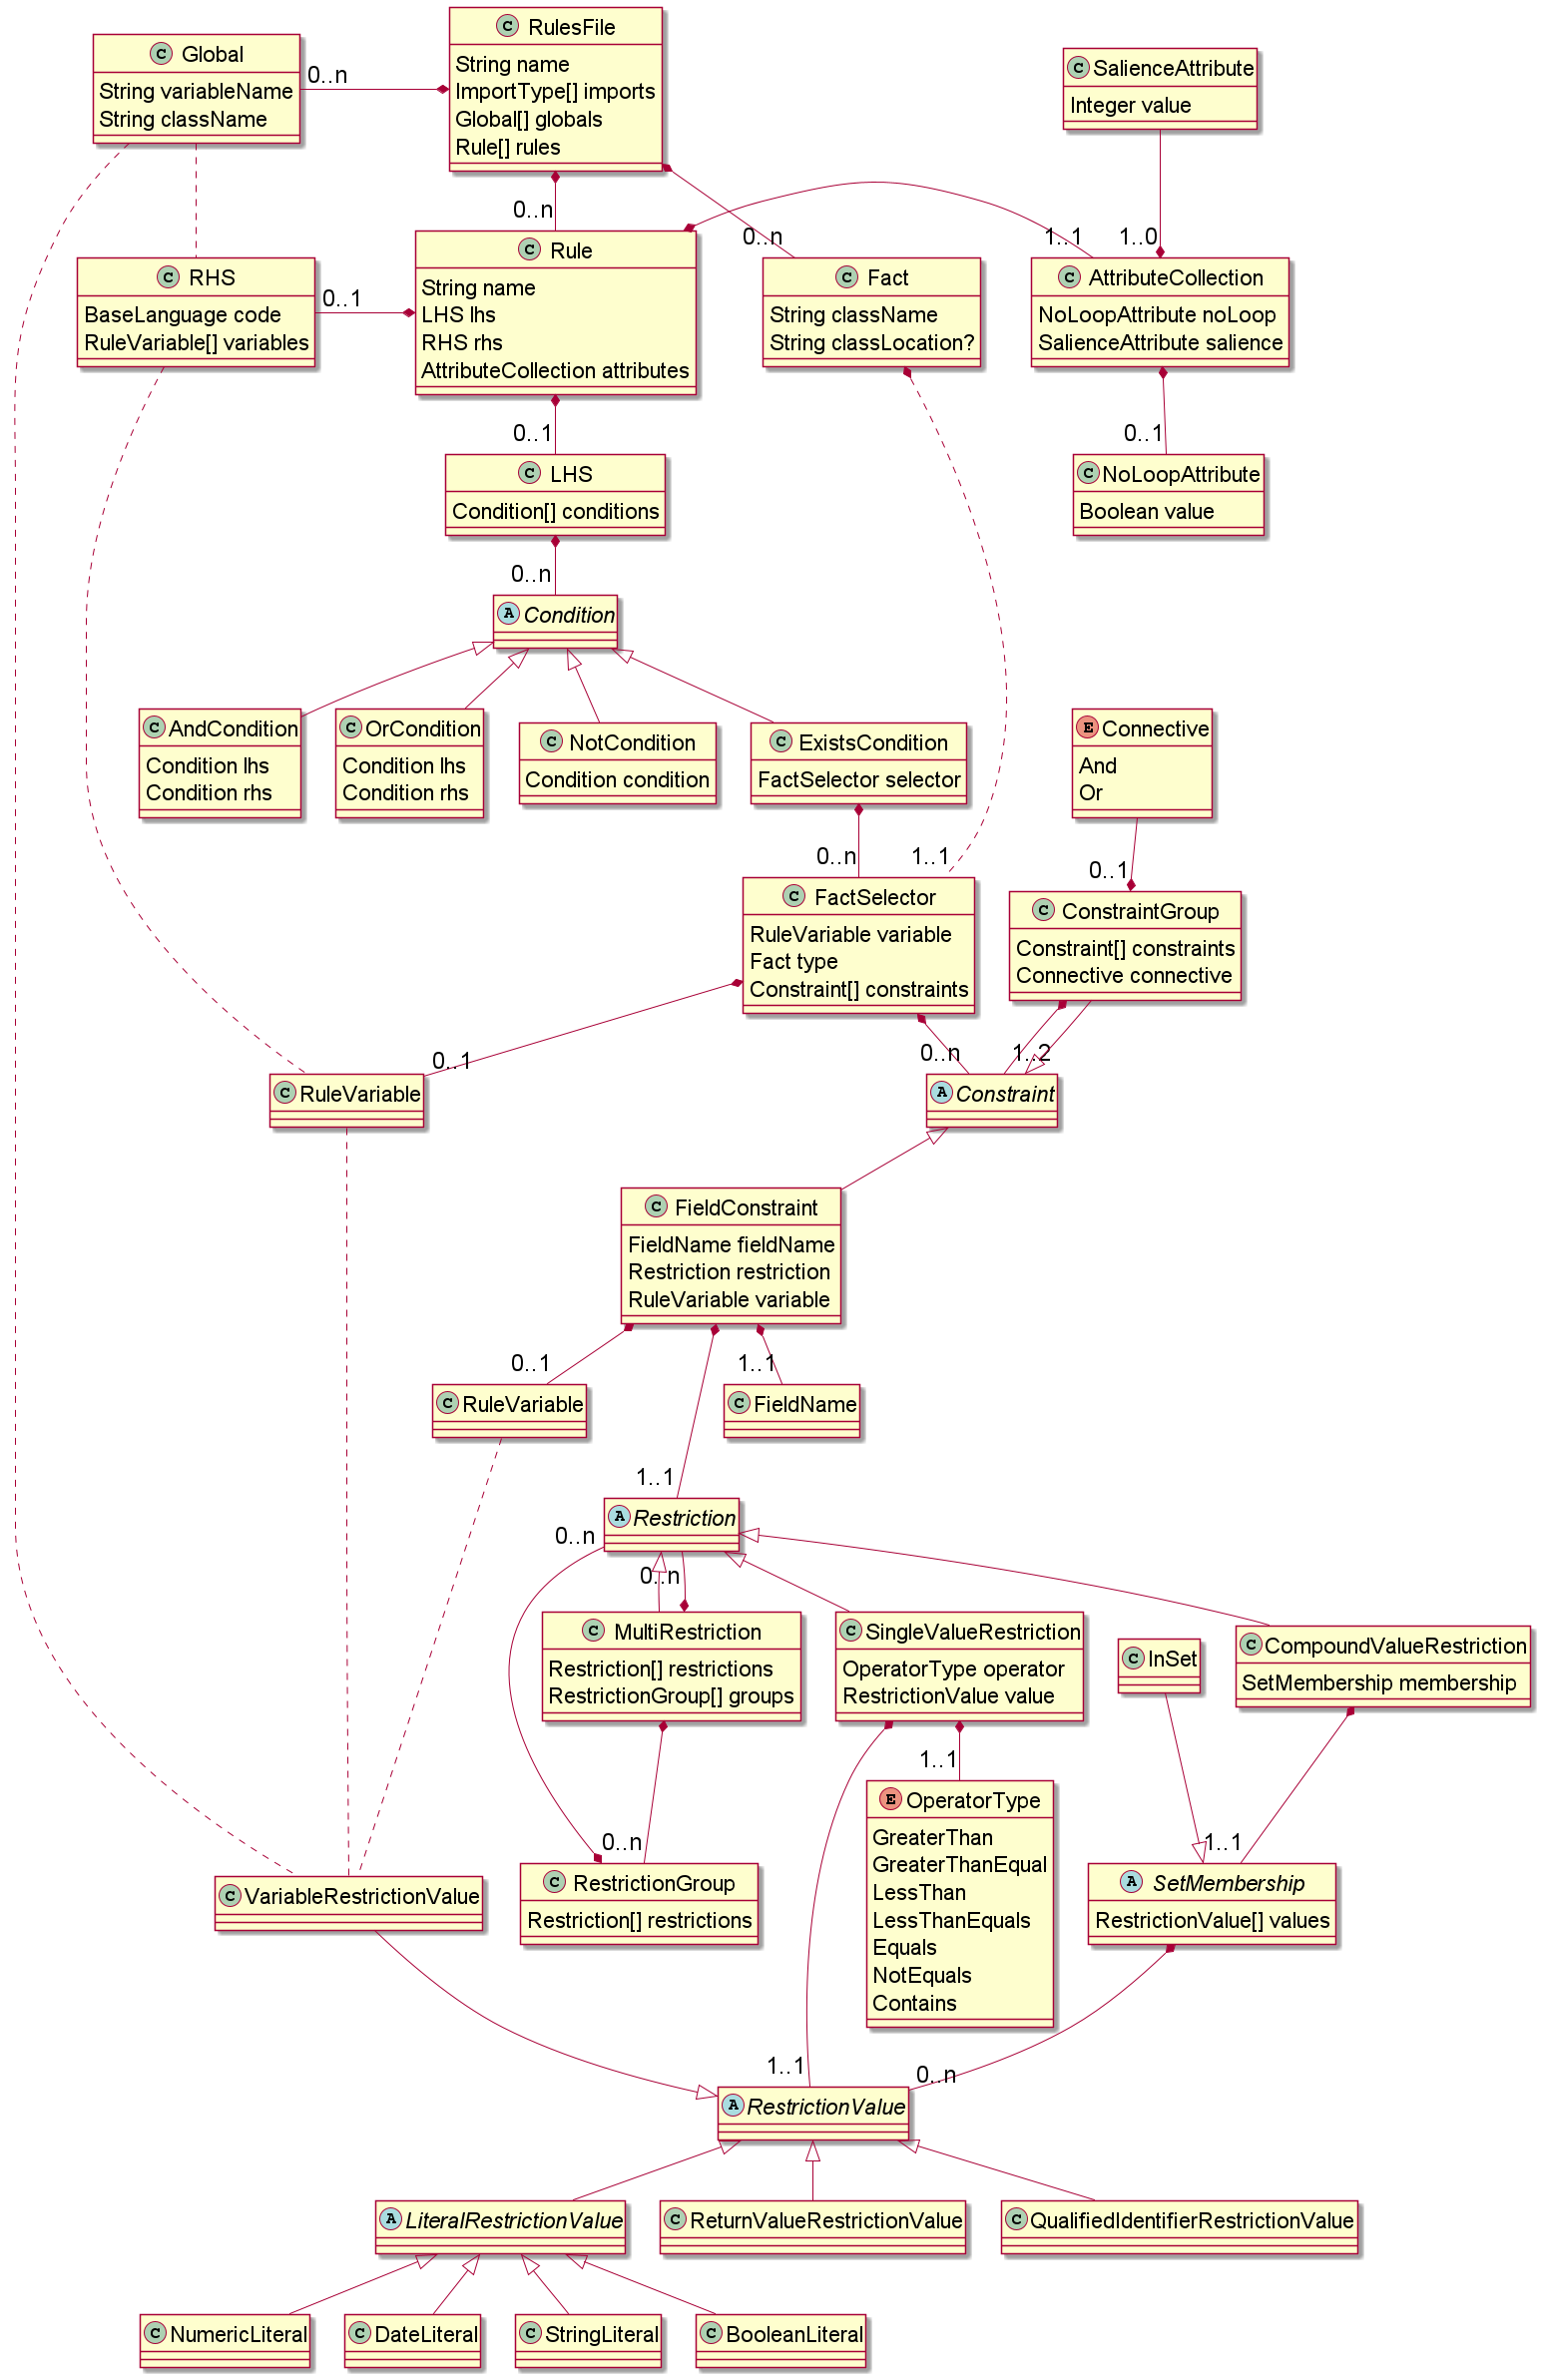
\includegraphics[width=0.85\textwidth]{Sections/images/DroolsLiteStructure.png}}
    \caption{Drools Lite Structure}
    \label{fig:DroolsLiteDiagram}
\end{figure}
\newpage
\section{Method: Survey}\label{section:Method_survey}
The validity of the the Prototype was tested using a survey.
If a survey is not well designed then it could lead to invalid or irrelevant outcomes.
As well as describing the design and procedure of the survey, we also outline any threats to its validity in this chapter.
Our choice of survey technique is a Questionnaire.

\subsection{Questionnaire Design}
The questionnaire can be found in appendix \ref{Appendix:Questionaire_text}.
To design the survey of our prototype, we followed a number of rules derived from the works of Bryman\cite{bryman2016social} and de Vaus\cite{de2013surveys}.

As advised, first we devised a clear introduction to describe the research.

We considered existing questions.
With regards to projectional editing, we requested the original questionnaires from three papers\cite{meacham2020adaptivevle,berger2016efficiency, voelter2014towards} pertaining to tools developed using projectional editing.
From these questionnaires we found [X] that we considered and decided against using any of them.

When formulating the questions we had the specific research question ``Which projections can help developers to get appropriate feedback about rules?'' in mind.

The pool of Drools users that we were personally in contact with was incredibly small.
Thus we had to rely on responses from strangers.
For this reason, we tried to make the questionnaire as quick to finish as possible.
This meant we looked particularly hard at removing questions that did not help us to our research goal.

We piloted the questionnaire with both ourselves and our industrial supervisor.

The instructions to each of the questions were tested for clarity, by a non-technical third party.

The only open question was one for which we wished to extract sentiment.
Rather than having yes/no questions, where appropriate we applied a Likert scale\cite{likert1932technique}.

The design of survey monkey layout makes sure that questions do not span pages.

The socio-demographic questions (skill level and experience) were left to the end and research based questions were toward at the beginning.

We took care to rework questions that were long, ambiguous, general, or leading to not be so.
We also took care to remove jargon, negative wording, and questions that asked about more than one thing.

\subsection{Participants}

The requirement for participants is that they have at least a little experience with using Drools.
It was our hope to get a statistically significant number of participants.

\subsection{Validity}
Non-response bias\cite{armstrong1977estimating} will be addressed by making the questionnaire short and easy to answer.
Because of the nature of the participant selection for this survey, it will be difficult to address the bias of self selection caused by voluntary response.

Common method bias, i.e. ``variance that is attributable to the measurement method rather than to the construct the measures represent''\cite{podsakoff2003common} can be responsible for 25\% or more of variable relational influence.
As we are only conducting a single survey, we won't be able to do much to prevent this, however we will take the following small precautions.
Testing the survey to remove question ambiguity, mood influences, and length issues.
Mixing the survey order of questions will be used to mitigate the issues caused by similarity of items, proximity of items, and location of items.
We will mitigate survey administration biases by administering some of these questionnaires manually and some online.
We will make sure that there are no right or wrong answers and aim toward fact based questions.
We will vary the scales of our Likert scales and the types of questions.

The main statistical methods to address this bias, i.e. ``Harman's single factor test''\cite{podsakoff2003common} and the``marker variable''\cite{lindell2001accounting} were found to be lacking in grounding\cite{gorrell2011countering}.
Marker variable is considered appropriate if used with caution.
With the size of our expected returns, it may not be possible to gain a statistically significant outcome.

\subsection{Pre-test}
The first attempt at the survey was sent to our industrial supervisor, who has experience with Drools.
We used this to remove ambiguously worded or leading questions and test that the length was truly between 5-10 minutes.
This lead to the following changes:
[TODO: add changes after we have tested]


\subsection{Sampling}
As within our own professional network we only had acquaintance with (6?) Drools developers, we had to expand our reach to those we did not personally know.

Our approach was first search StackOverflow for question askers and answerers on the subject of Drools.
Our preference was to find email addresses, failing that twitter contacts.
This proved to be quite limited, especially in attempting to get contact details, 13 email addresses and 6 twitter addresses.

Our next approach was to trawl our LinkedIn connections for anyone with drools as a proclaimed skill.
Whilst we had no one in our direct contacts, at one level of separation we found 204 connections.
From these we could extract 54 email addresses and 40 twitter addresses, with only a small crossover with the addresses harvested from StackOverflow.

We chose not to expand to third level contacts, as we thought this would be harder to sell as to why they should feel comfortable answering us.

\subsection{Procedure}

The questions, as described in appendix \ref{Appendix:Questionaire_text}, was uploaded to Survey monkey.

To encourage response, especially amongst only tangentially known participants, we crafted a short introduction, using techniques designed to enhance response as discussed by amongst others Cialdini\cite{goldstein2008yes}.
As seen in figure \ref{fig:persuasive_introduction}, the attics discussed by Cialdini, as signposted in table \ref{table:persuasive_introduction}.
\begin{table}[h]
    \begin{center}
        \begin{tabular}{ |l | l |  } 
            \hline
            Key &  Tactic\\
            \hline
            1  & Short option for those with no time \\
            2  & Credentials matter \\
            3  & Recognition, (this might backfire as I hardly remember any of my LinkedIn connections) \\
            4  & Consistency, they reported they have Drools experience, so they must live up to it \\
            5a\&b  & Social Proof - other people have already answered \\
            6  & showing value \\
            7  & Special because of scarcity \\
            8  & Labelling - ``I see you to be a good person'' \\
            9  & The word ``Because'' has an outweighed effect \\
            10 & Compliment Expertise \\
            11 & ``Every little helps'' \\
            12 & point out a fault \\
            13 & own the fault \\
            14 & ask a favour \\
            15 & add inconvenience \\
            16 & Rhyming \\
            17 & hand written note \\
            \hline
        \end{tabular}
    \end{center}
    \caption{persuasion tactics in figure \ref{fig:persuasive_introduction}}
    \label{table:persuasive_introduction}
\end{table}

\begin{figure}[h]
    \centering
    \fbox{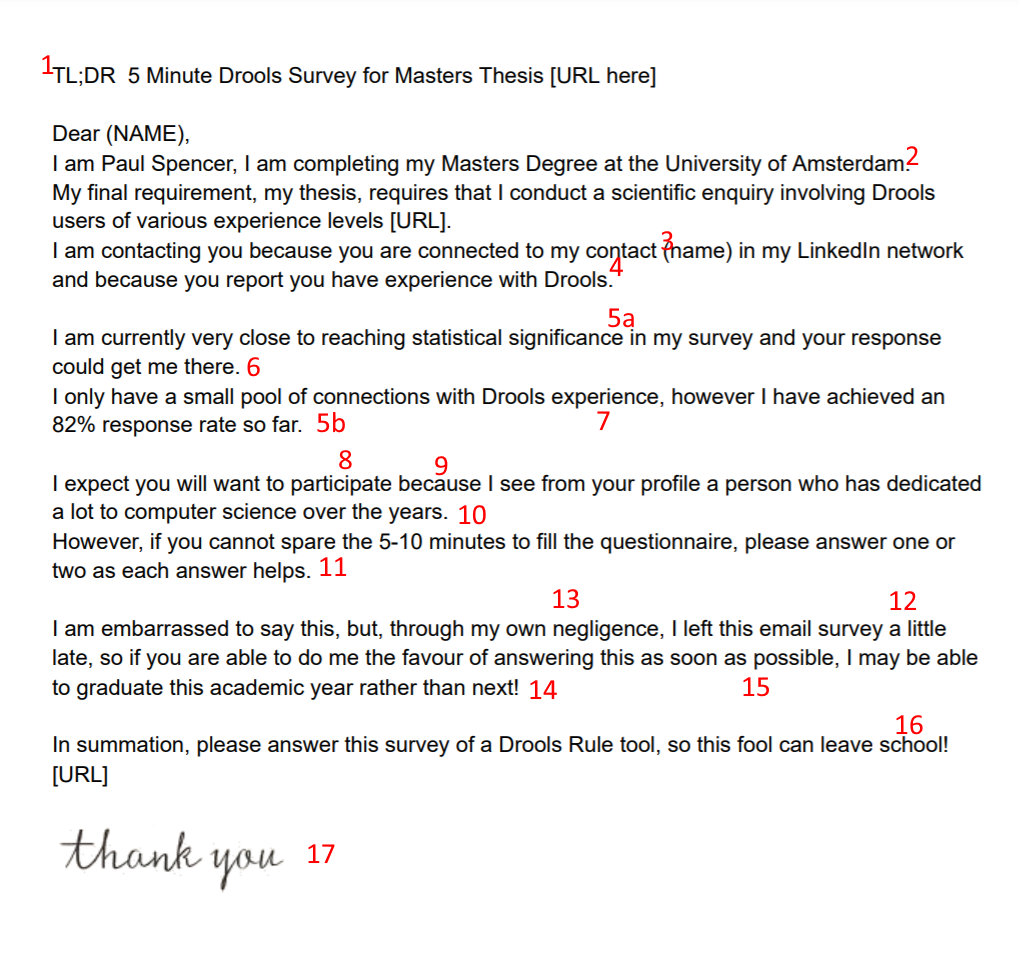
\includegraphics[width=0.85\textwidth]{Sections/images/persuasion.png}}
    \caption{persuasive introduction.}
    \label{fig:persuasive_introduction}
\end{figure}

These were sent to our list of drools using strangers and we sat back and awaited response.
